% GCIS ESIP talk

\documentclass{beamer}
\usepackage{lmodern}
%\documentclass[notes=only]{beamer}
\usepackage[T1]{fontenc}

\usepackage{fancyvrb}
\usepackage{graphicx}

\setbeamertemplate{navigation symbols}{}
\usetheme{Boadilla}
\usecolortheme{dove}
\beamersetuncovermixins{\opaqueness<1>{25}}{\opaqueness<2->{15}}
\setbeamertemplate{itemize items}[circle]
\setbeamertemplate{enumerate items}[default]
\setbeamertemplate{section in toc}{\inserttocsectionnumber.~\inserttocsection}
\setbeamercolor{subsection in toc}{bg=white,fg=structure}
\setbeamertemplate{subsection in toc}{%
 \hspace{1.3em}{
     \boldmath$\cdot$
  }~\inserttocsubsection\par}

\AtBeginSection[]
{
\begin{frame}<beamer>
  \frametitle{Outline}
  \tableofcontents[currentsection]
\end{frame}
}


\begin{document}
\title[Global Change Information System]{Adaptable Information Models in the\\
Global Change Information System}
\author[Duggan et al]{
    Brian Duggan\inst{1}\inst{2},
    Andrew Buddenberg\inst{3}, \\
    Steve Aulenbach\inst{1}\inst{2},
    Robert Wolfe\inst{1}\inst{4},
    Justin Goldstein\inst{1}\inst{2}
}
\date{December 16, 2014} 
\institute[USGCRP, UCAR]{
\inst{1} US Global Change Research Program \\
\inst{2} University Coporation for Atmospheric Research \\
\inst{3} National Oceanic and Atmospheric Administration \\
\inst{4} National Aeronautics and Space Administration
}

% \begingroup
% \makeatletter
% \setlength{\hoffset}{-.5\beamer@sidebarwidth}
% \makeatother
% \endgroup

\begin{frame}[plain]
\titlepage
\begin{center}
\url{http://data.globalchange.gov}\\
\url{http://github.com/USGCRP/gcis}
\end{center}
\end{frame}

\begin{frame}
\frametitle{Outline}
\tableofcontents 
\end{frame}

\section{Introduction and Functionality}

\subsection{Overview}
\frame{
    \frametitle{\insertsubsectionhead}
    The US Global Change Research Program (USGCRP) has established
    the Global Change Information System (GCIS) to better coordinate
    and integrate the use of Federal information products on changes
    in the global environment and the implications of those changes for society.
}
\frame{
    \frametitle{\insertsubsectionhead}
    The GCIS provides a RESTful API for retrieving global change information.\\
    The GCIS also provides a triple store.  URLs in the triple store are resolvable
    using the API.  URIs in the triple store are described by the GCIS ontology.
}

\subsection{Producing the Third National Climate Assessment}

\frame{
    \frametitle{\insertsubsectionhead}
    In May, 2014, the US Global Change Research Program released
    the 2014 National Climate Assessment.\\
    \medskip
    Production of this 829 page report and its web site involved collaboration between
    over 300 authors, numerous editors, graphics producers, scientists, data scientists,
    software developers, and web teams.\\
    \medskip
    The content included 161 findings, 284 figures, 3,395 bibliographic references (journal
    articles, books, reports).\\
    \medskip
     The GCIS facilitated the assembly of the report by providing common {\bf identifiers} for
     resources and concepts, providing a common web interface for entering and viewing information,
     as well as an API for adding and removing information using a variety of formats.
\note{Endnote, Drupal, MS Word, Excel, Google Docs, Graphics Software}
}

\frame{
    \frametitle{\insertsubsectionhead}
    \begin{columns}
        \begin{column}{0.6\textwidth}
            \fbox{
            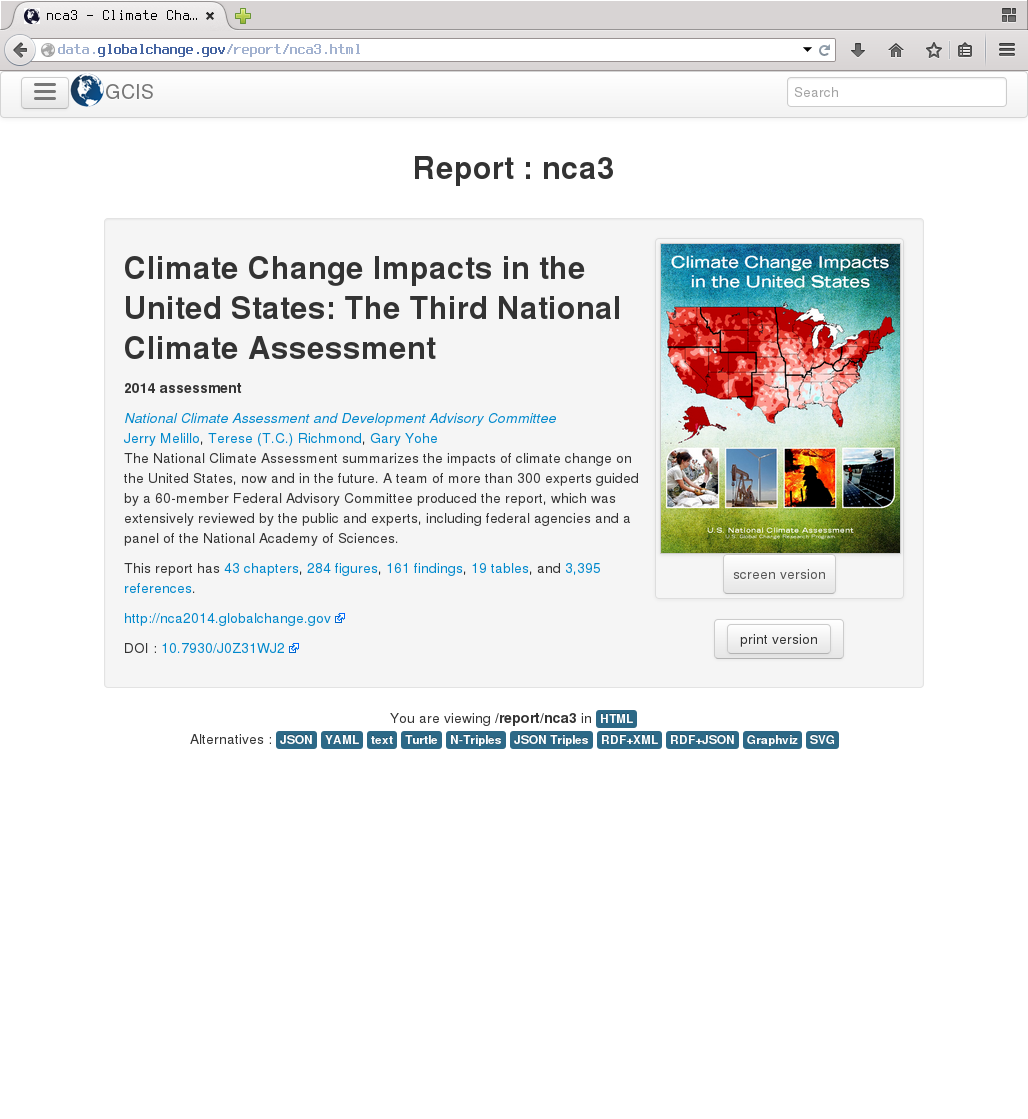
\includegraphics[height=0.8\textheight]{gcis-nca3.png}
            }
        \end{column}
        \begin{column}{0.4\textwidth}
            data.globalchange.gov\\
            /report/nca3\\
            .html
        \end{column}
    \end{columns}
    \note{The html is implicit but can be replaced with json (or yaml), ttl for turtle, or other rdf serializations like ntriples, rdf
        Also, /report/nca3 is the URI which we treat as the canonical identifier for this report.  We do the same for other objects
        like chapters, references, figures, findings, authors.
        }
}


\subsection{Supporting the NCA3 website}
\frame{
    \frametitle{\insertsubsectionhead}
    
            A website, \url{http://nca2014.globalchange.gov}, was released concurrently with the report.
            The site received over 200,000 visits in the first two days after launch and continues to
            receive frequent main stream media attention.\\
            \medskip
            GCIS serves as the backend : the website sends client side requests to \url{http://data.globalchange.gov}
            and receives JSON responses which it uses to populate elements of some pages dynamically.\\

}

\frame{
    \frametitle{\insertsubsectionhead}
    \centering
    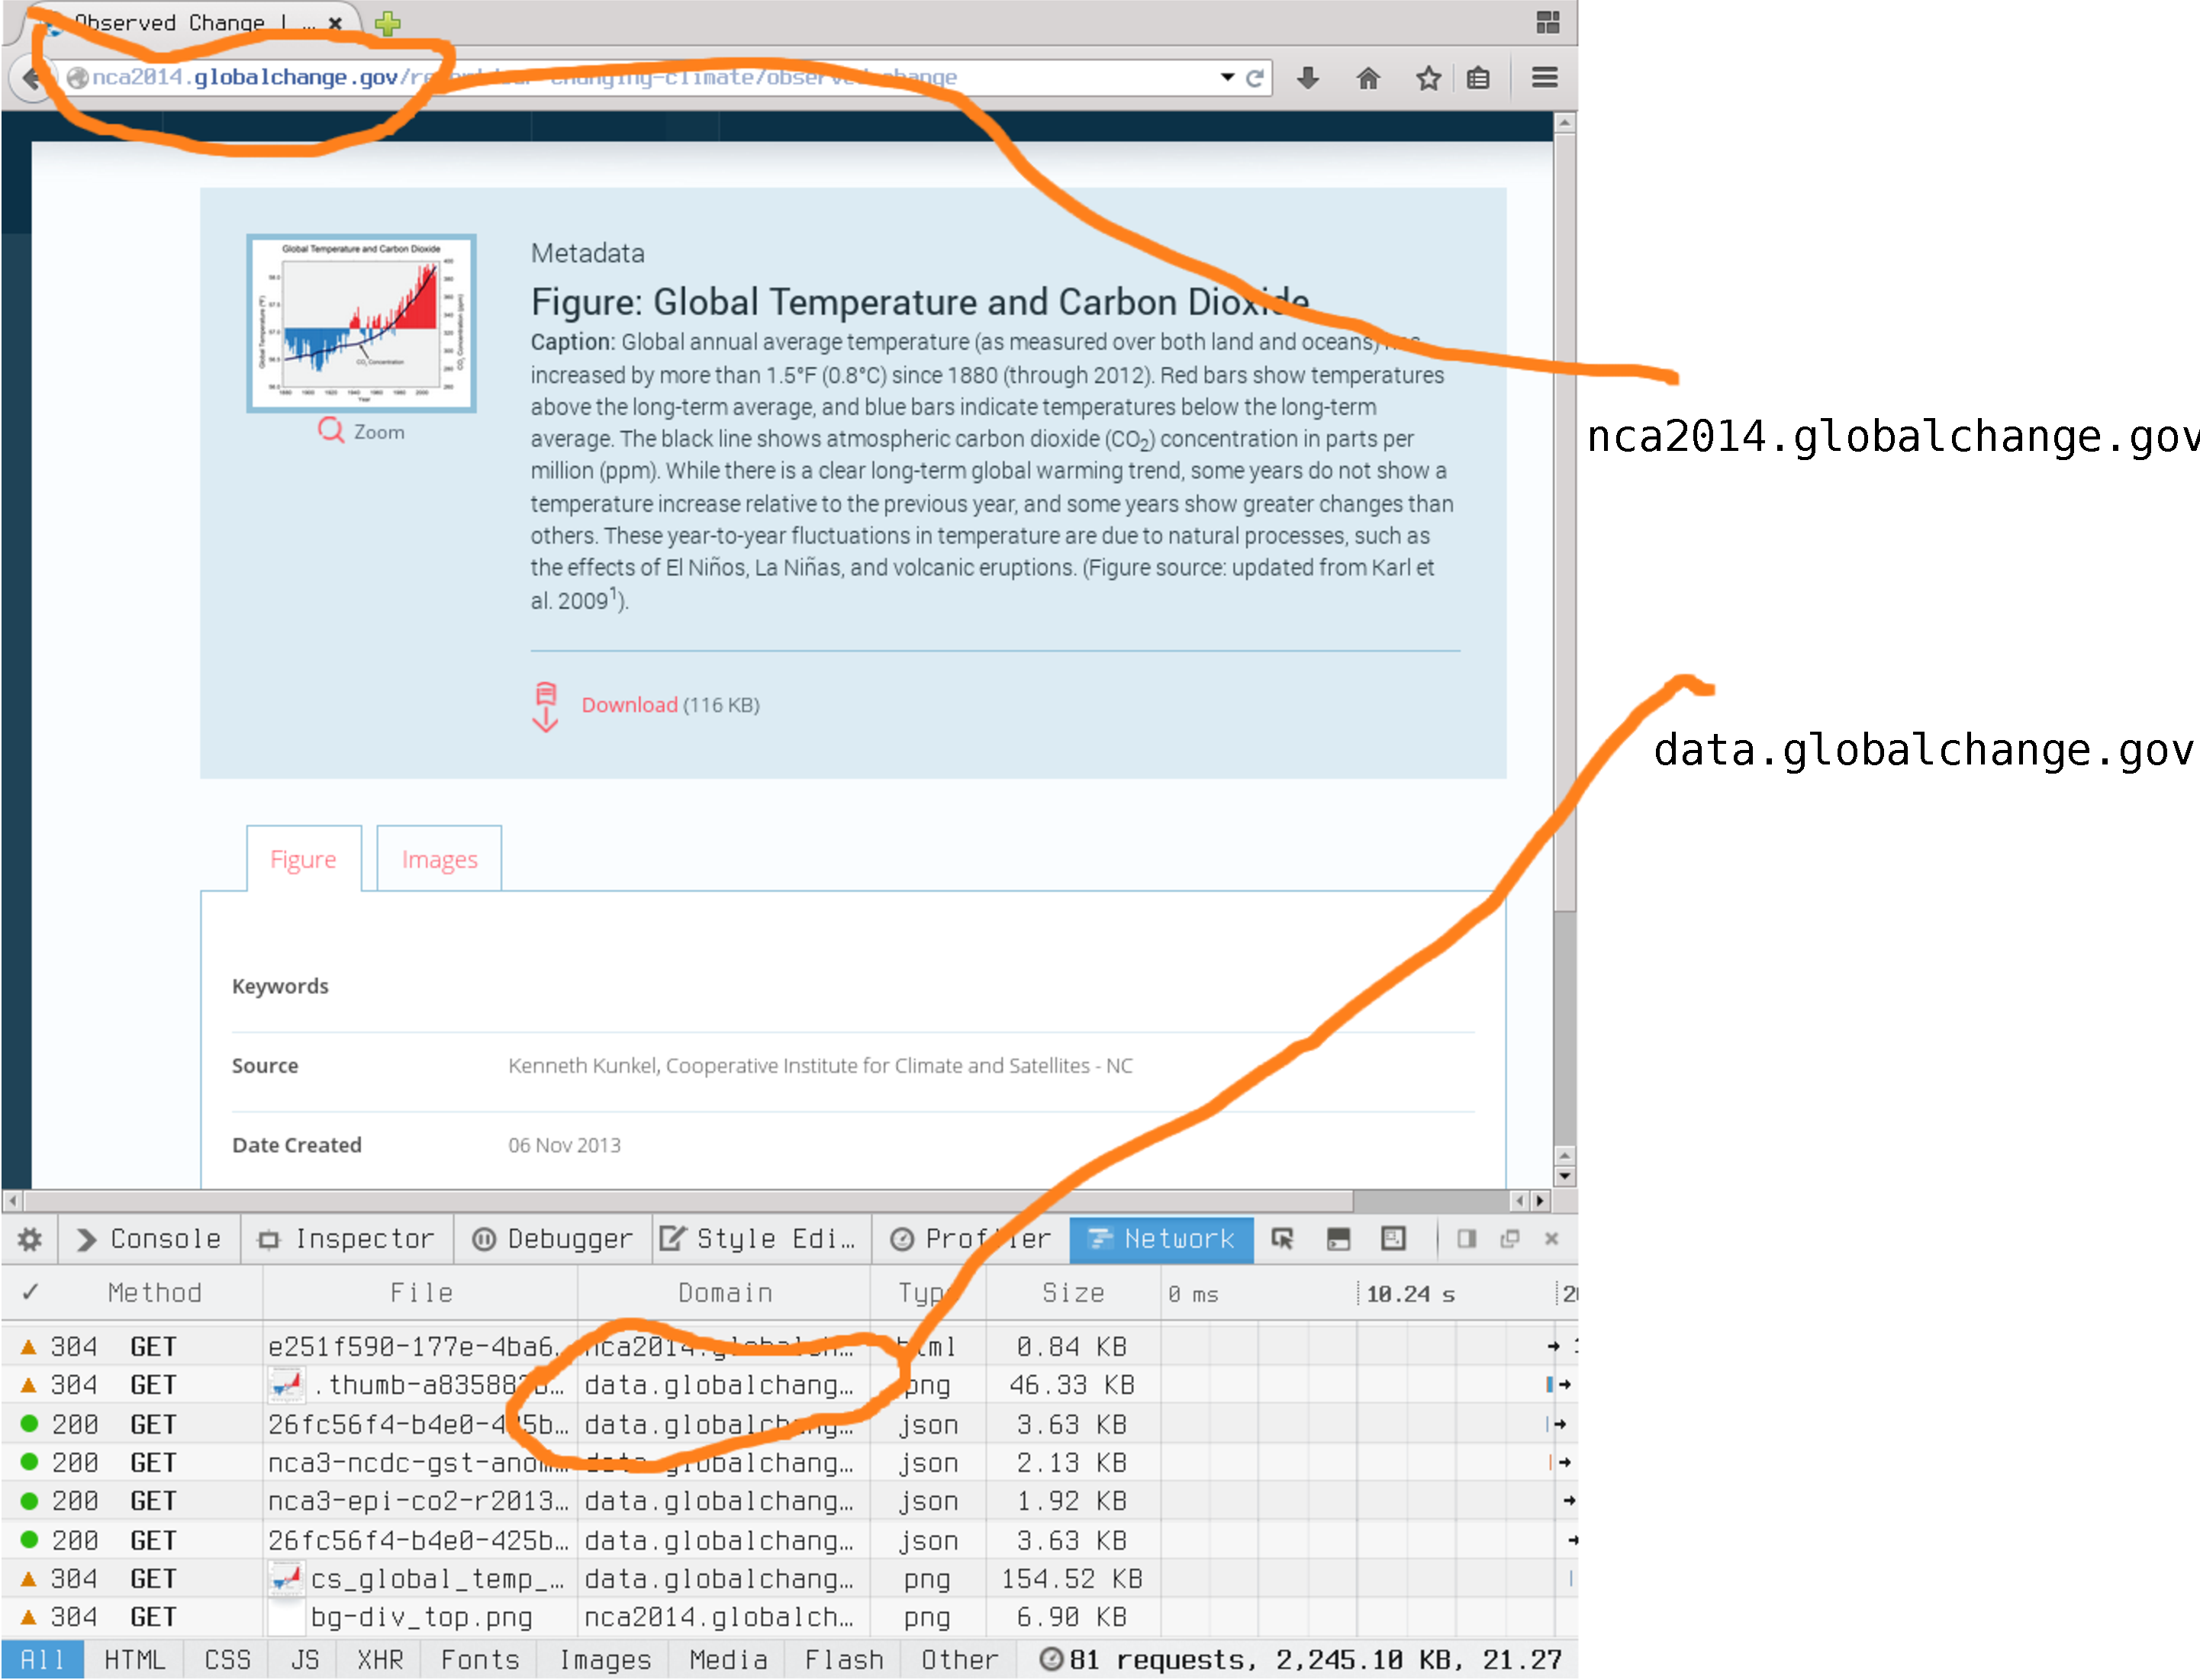
\includegraphics[height=0.9\textheight]{ncaweb-drawn.pdf}
}

\subsection{Provenance}
\frame{
    \frametitle{\insertsubsectionhead}
    The identifiers within GCIS can be used to trace the provenance of figures, findings, and other resources.\\
    \medskip
    A figure may be derived from a journal article which is derived from a dataset which is derived from a NASA standard
    product which is derived from an instrument which is on a platform.
}

\frame{
    \frametitle{\insertsubsectionhead}
    \begin{center}
    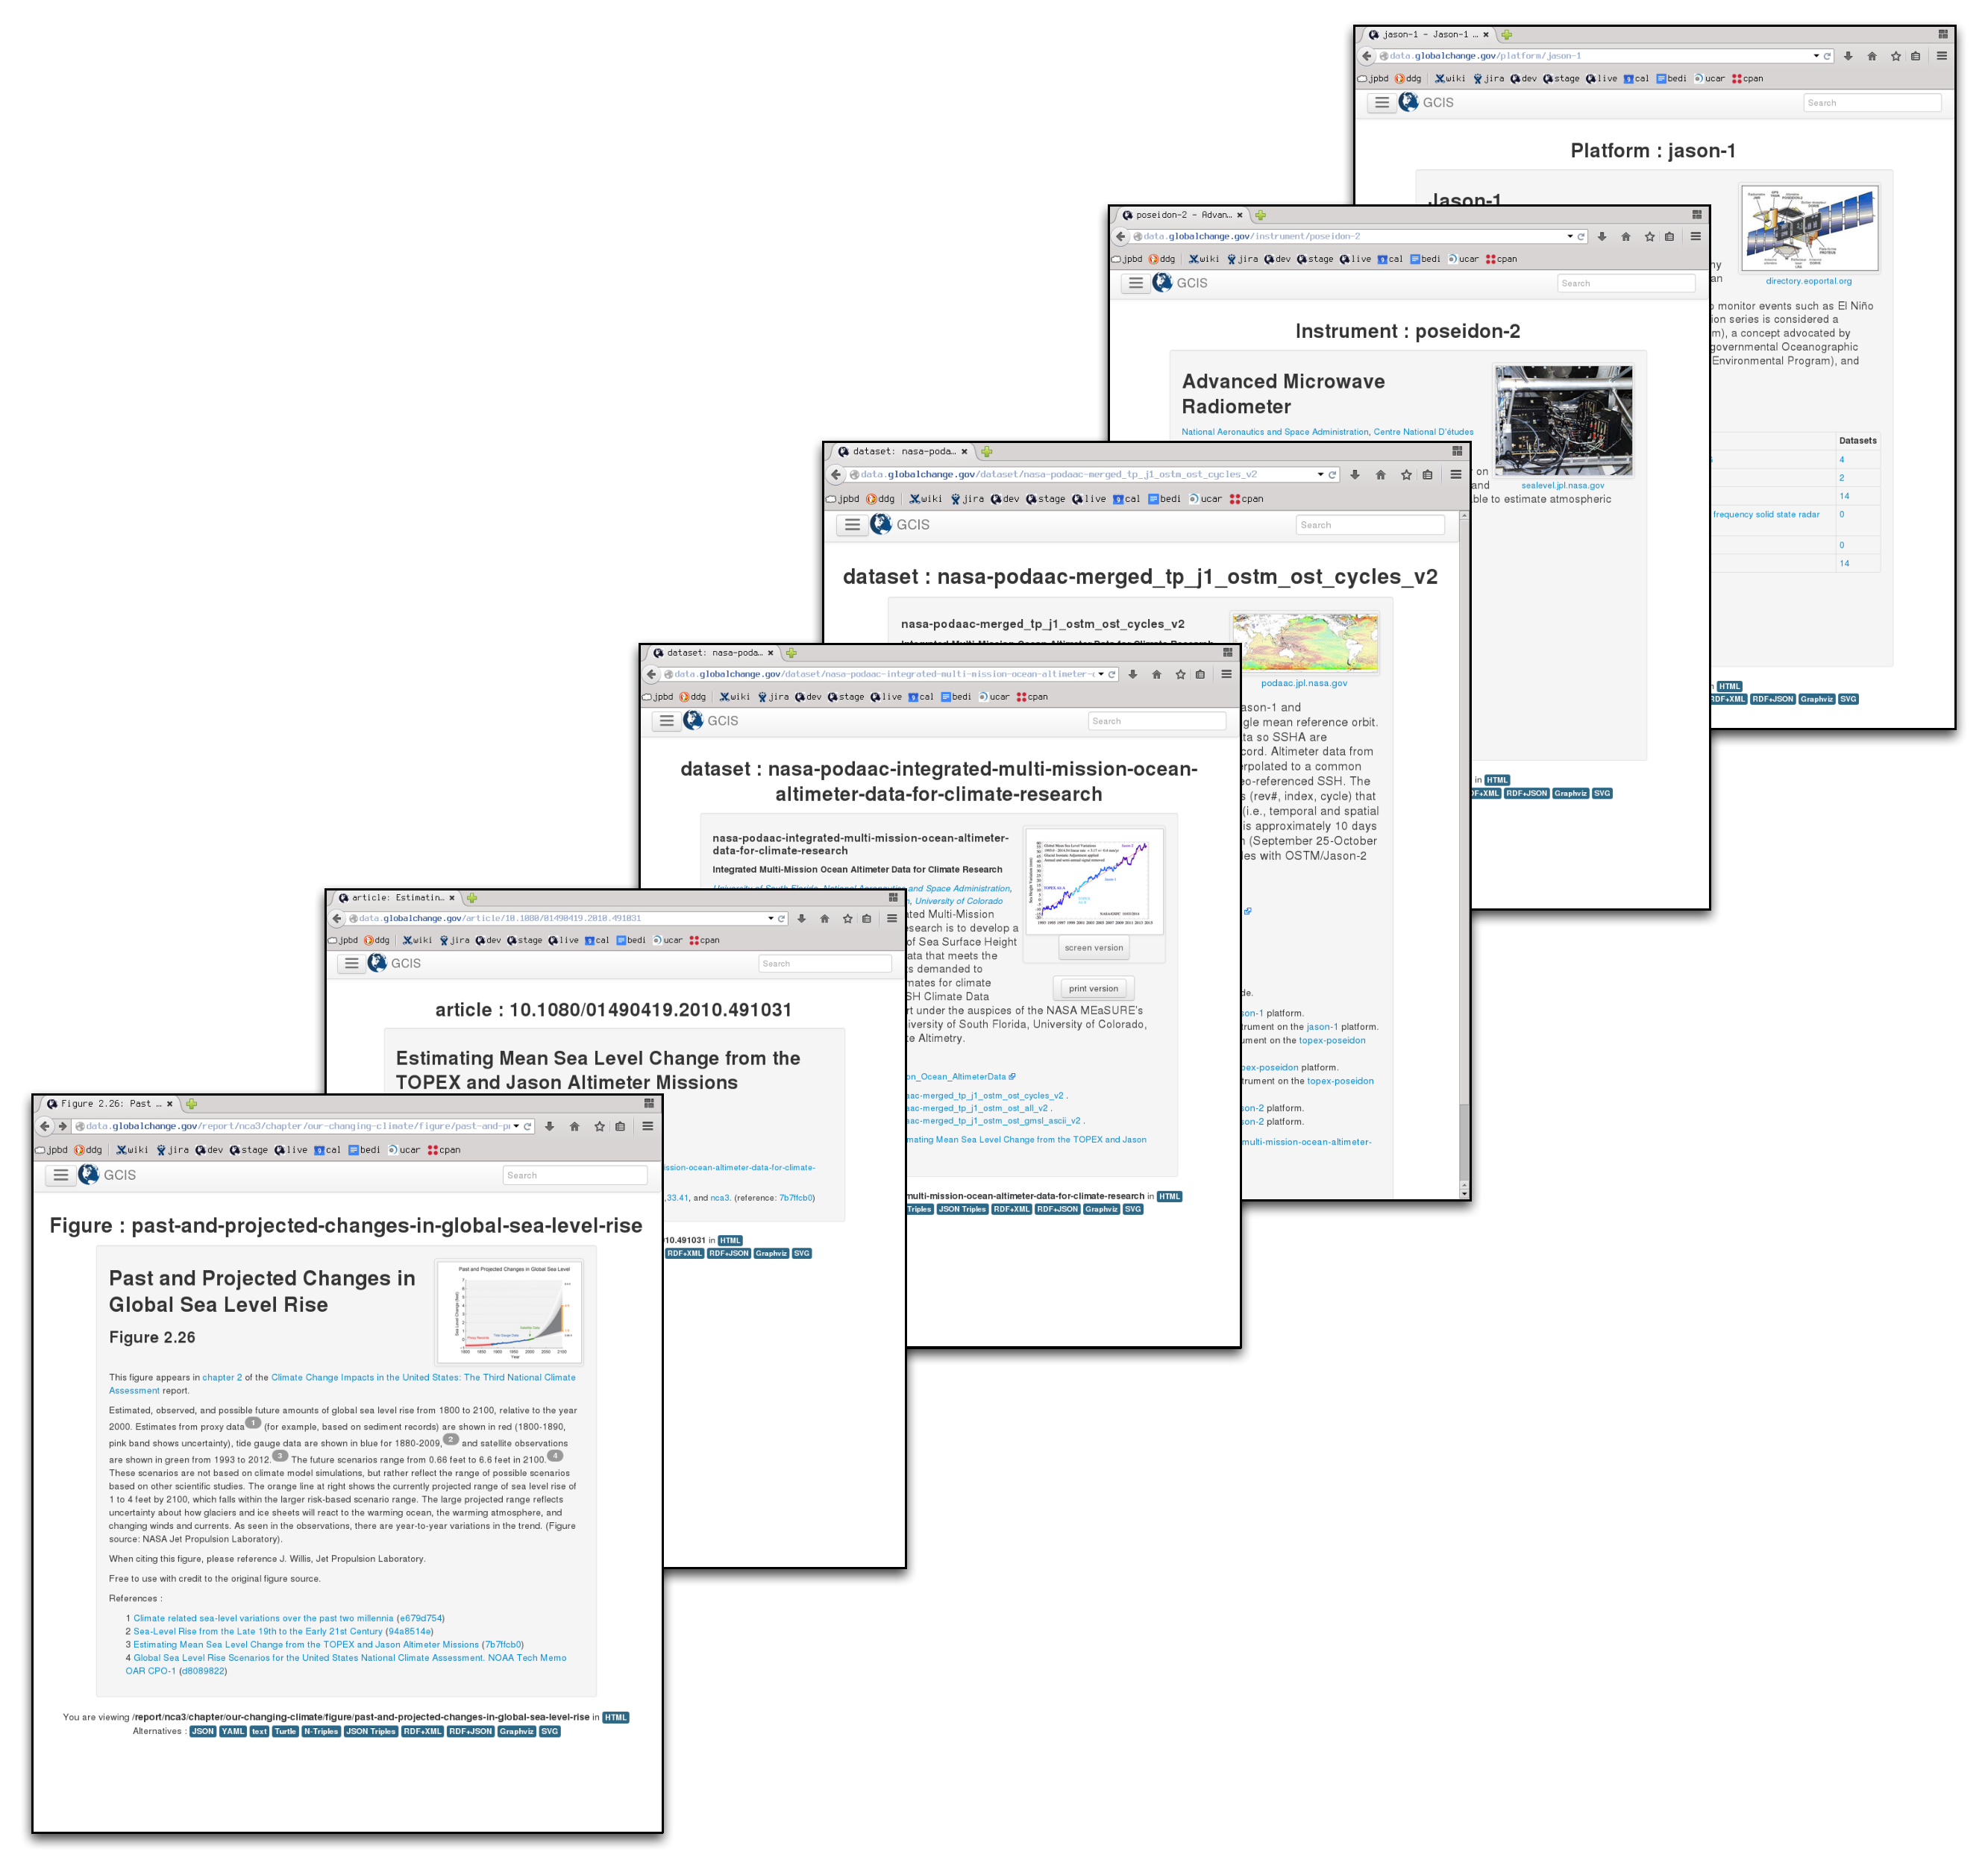
\includegraphics[height=0.9\textheight]{sealevel/figure-to-platform.pdf}
    \end{center} 
}


\subsection{Queries}
\frame{
    \frametitle{\insertsubsectionhead}
    Structured information allows for querying.
    \medskip
    \begin{itemize}
        \item Find reports with figures derived from a dataset generated by an instrument on a specific platform.
        \item Show figures associated with data generated by instruments on platforms flown by NOAA.
    \end{itemize}
    Queries are based on the information model.
}

%% tech
\section{Information Model}
\subsection{Relational}
\frame{
    \frametitle{\insertsubsectionhead}
    Canonical representation : PostgreSQL database.\\
    \begin{itemize}
        \item One-many, many-one, many-many relationships.
        \item Referential integrity.
        \item String type checking.
        \item Column constraints.
        \item Cascading updates and deletes.
        \item Well known optimization techniques.
        \item Wide spread adoption.
    \end{itemize}
    PostgreSQL hstores allow key-value storage.\\
    \medskip
    Closed world assumption.
    \note{Closed world : A figure is related to a chapter if and only if that relationship is present.}
    \note{Postgres also has some things like hstores for occasional key-value storage.}
}

\subsection{Semantic}
\frame{
    \frametitle{\insertsubsectionhead}
    \begin{itemize}
        \item Relationships are first class objects.
        \note{not just 1-1 or 1-many or many-1 or many-many}
        \item Concepts are formally defined in an ontology.
        \item Formal definitions help remove ambiguities.
        \note{There is no requirement for definitions in a relational model.  What is a figure?  What is an image?}
        \item Interoperability with other systems.
    \end{itemize}

    Open world assumption.
    \note{Just because a fact is missing does not mean it is false.}
}

\subsection{Example}
\begin{frame}[fragile]
    \frametitle{\insertsubsectionhead}
     \url{http://bit.ly/gcis-dbpedia}\\
\begin{tiny}
\begin{Verbatim}
    PREFIX bibo: <http://purl.org/ontology/bibo/>
    PREFIX gcis: <http://data.globalchange.gov/gcis.owl#>
    PREFIX cito: <http://purl.org/spar/cito/>
    PREFIX dcterms: <http://purl.org/dc/terms/>
    PREFIX dbprop: <http://dbpedia.org/property/>
    PREFIX dbpo: <http://dbpedia.org/ontology/>

    SELECT  DISTINCT ?dbpjournal ?gcisjournal ?issn
    FROM <http://data.globalchange.gov>
    WHERE {
       SERVICE <http://data.globalchange.gov/sparql> {
            ?gcisjournal a bibo:Journal .
            ?gcisjournal bibo:issn ?issn .
            ?gcisjournal dcterms:hasPart ?gcisarticle .
            ?gcisarticle a bibo:Article .
            ?gcisarticle dcterms:isPartOf ?gcisjournal .
            ?gcisarticle cito:isCitedBy <http://data.globalchange.gov/report/nca3> .
       }
       SERVICE <http://dbpedia.org/sparql> 1
        ?dbpjournal dbprop:frequency "Monthly" @en .
        ?dbpjournal dbpo:issn ?issnd .
       }
       FILTER(?issnd = ?issn)
    }
\end{Verbatim}
\end{tiny}
    Find monthly journals which have had an article cited by the NCA3 report.

\note{Note : GCIS does not store the frequency of publication of a journal.
    But it does store the ISSN, and dbpedia stores the frequency.
    So, it's possible to join GCIS to dbpedia to use this attribute.  Go to
    the URL bit.ly/gcis-dbpedia to actually run this query.}
\end{frame}

\section{System Architecture}

\subsection{Diagram}

\frame{
    \frametitle{\insertsubsectionhead}
    todo
}

\subsection{Content Changes}
\frame{
    \frametitle{\insertsubsectionhead}
    When identifiers exist in other APIs, we can match them with
    GCIS identifiers, to perform updates.\\
    For journal articles, use DOIs and crossref.org.\\
    When identifiers are unique to specific organizations, maintain
    a table which maps organization identifiers to GCIS identifiers.\\
    We call these tables lexicons.\\
    Example :\\
    PO.DAAC has identifiers for satellites.  So does CEOS.  Map both
    to GCIS identifiers.\\
    PODAAC : AQUA -> /platform/aqua\\
    CEOS : 206 -> /platform/aqua\\
    Allows PODAAC identifiers to be mapped to CEOS identifiers.
}
\subsection{Schema Changes}

\frame{
    \frametitle{\insertsubsectionhead}
    Changes to the schema propagate to the JSON API.
    JSON key names match the column names, and nested JSON objects correspond to relationships.
    \begin{enumerate}
        \item Write a test for new REST functionality.
        \item Run the tests.  Do they test pass?
        \item Yes?  Done.
        \item No?  Write a schema patch.
        \item Goto step 2.
    \end{enumerate}
    The tests remain part of the test suite, which is run continuously.
    \note{This is the typical methodology for test driven development.  But the implicit
    magic is that running the tests involves patching the database schema on a fresh instance,
    and starting the application.}
}

\subsection{Ontology Changes}
\frame{
    \frametitle{\insertsubsectionhead}
    Change to the triple are handled by turtle templates.
    \begin{enumerate}
        \item Write a test with a SPARQL query that should succeed.
        \item Run the tests.  Do they pass?
        \item Yes?  Done.
        \item No?  Modify the turtle templates.
        \item Go to step 2.
    \end{enumerate}
    The tests remain part of the test suite, which is run continuously.
    \note{This is again the typical test drive development flow.  Here the implicit
        magic is that the test suite constructs a temporary triple story which can
        be queried with SPARQL.}
}
\begin{frame}[fragile]
    \frametitle{\insertsubsectionhead}
    Sample turtle template :
    \begin{Verbatim}[commandchars=\\\{\}]
    {\bf <%= article->uri %>} a gcis:Article;
    {\bf <%= article->uri %>} dcterms:isPartOf
        {\bf <%= article->journal->uri %>};

    \end{Verbatim}
\end{frame}

\section{Conclusion, Ongoing Work, Future Plans}

\frame{
    \frametitle{\insertsubsectionhead}
Current work involves extending the data model to include models, in situ observations,
datasets from more DAACs, and identifying lexicons and APIs for GCIS resources.
}

\frame{
    \frametitle{Thank you}
    http://github.com/usgcrp/gcis\\
    http://data.globalchange.gov\\
    http://www.globalchange.gov
}

\end{document}

